\section{Results and Discussion}

After simulating all possible combinations of algorithm, agent policy, and traffic density, the global metrics were collected and are summarized in the table below:

\begin{figure}[H]
    \centering
    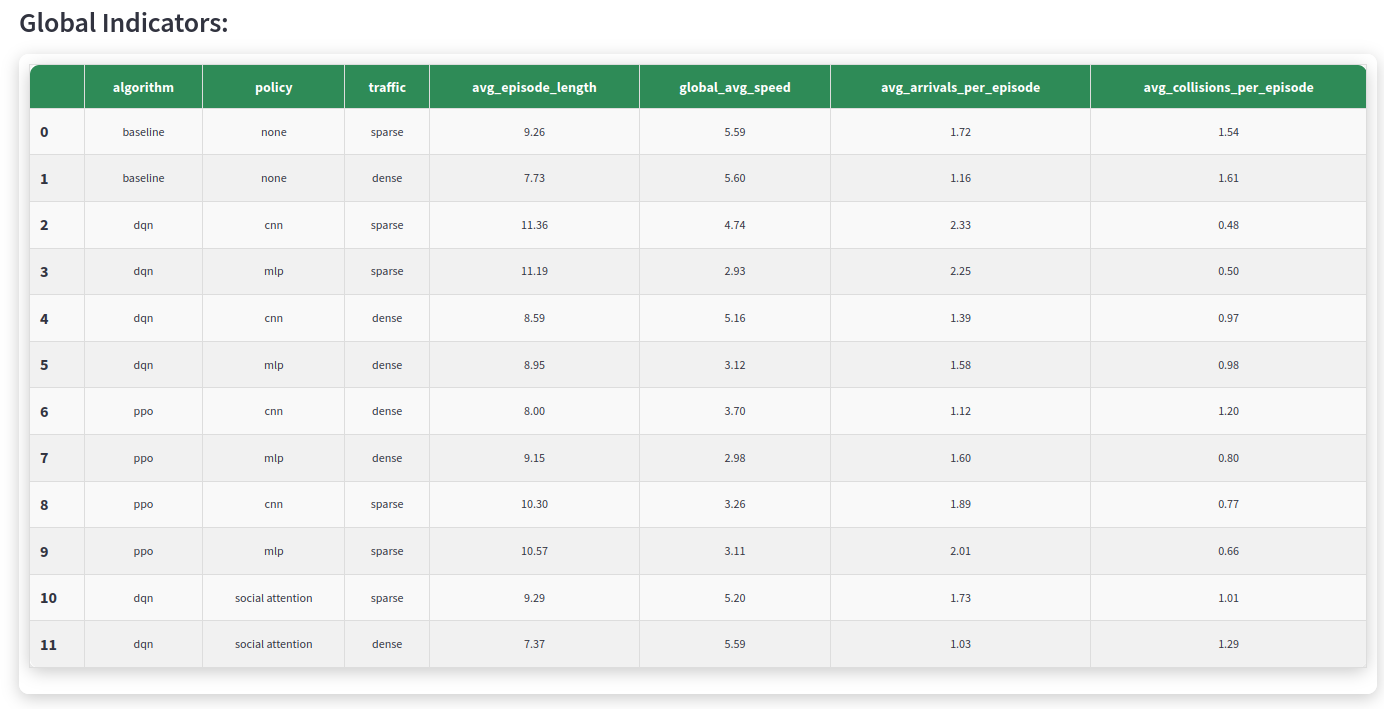
\includegraphics[height=0.38\textheight]{images/app_global_indicators.png} 
    \caption{Summary of Global Metrics for All Algorithm / Policy / Traffic Combinations}
\end{figure}

and plotted:

\begin{figure}[H]
    \centering
    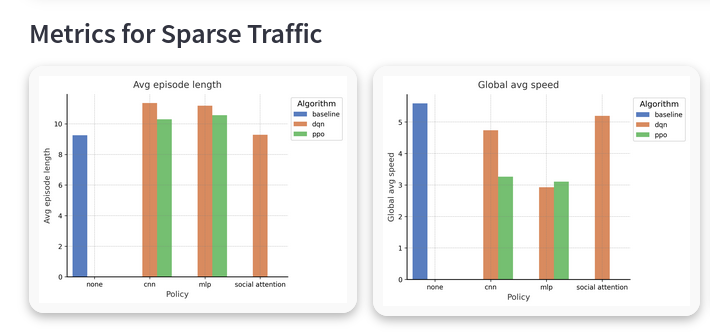
\includegraphics[height=0.215\textheight]{images/app_global_plots_sparse1.png} 
\end{figure}

\begin{figure}[H]
    \centering
    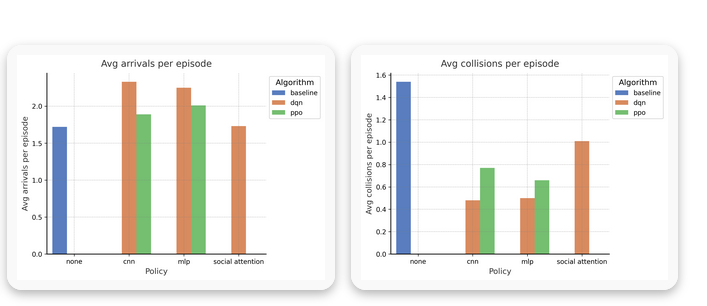
\includegraphics[height=0.2\textheight]{images/app_global_plots_sparse2.png} 
    \caption{Summary of Global Metrics for Sparse Traffic}
\end{figure}

\begin{figure}[H]
    \centering
    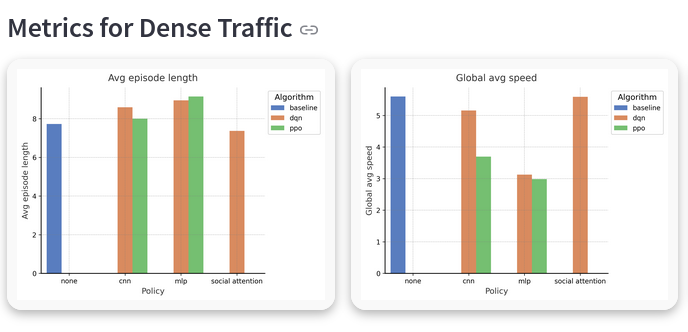
\includegraphics[height=0.215\textheight]{images/app_global_plots_dense1.png} 
\end{figure}

\begin{figure}[H]
    \centering
    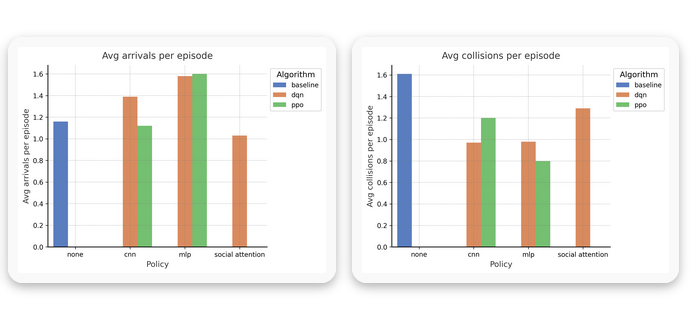
\includegraphics[height=0.2\textheight]{images/app_global_plots_dense2.png} 
    \caption{Summary of Global Metrics for Dense Traffic}
\end{figure}

The results in the table reveal several important trends and insights regarding the performance of the different combinations of algorithm, policy, and traffic density:

\subsection{Average Episode Length}

The average episode length is an important indicator of how well an algorithm handles the traffic conditions without causing early terminations (such as collisions). A longer episode typically suggests that the algorithm is performing well by effectively navigating through the environment, handling traffic without triggering collisions, while shorter episodes may indicate that the agent fails to handle the traffic complexity and encounters more collisions, which results in the early termination of the episode.

From the table, we can observe the following trends in episode length:

\begin{itemize}
    \item The \textbf{baseline} algorithm with the \textbf{none} policy shows relatively shorter episode lengths in both sparse and dense traffic conditions (9.26 and 7.73, respectively). The relatively short episode lengths may suggest that the baseline algorithm struggles with maintaining stability in traffic environments and is prone to more frequent collisions, causing earlier episode termination.
    \item The \textbf{dqn} algorithm with \textbf{cnn} and \textbf{mlp} policies, particularly in sparse traffic, exhibits longer episode lengths (11.36 and 11.19, respectively). These longer episode durations suggest that deep reinforcement learning algorithms like DQN are better equipped to handle traffic without resulting in collisions, even in more unpredictable environments.
    \item In dense traffic, the \textbf{dqn} with \textbf{cnn} (8.59) and \textbf{mlp} (8.95) still shows moderate episode lengths, indicating that these algorithms can handle denser traffic effectively and extend the duration of episodes by avoiding early terminations.
    \item The \textbf{ppo} algorithm generally shows shorter episode lengths compared to DQN. Episode lengths range from 8.00 (cnn, dense) to 10.57 (mlp, sparse). The shorter episode lengths in some cases suggest that PPO might encounter more collisions, leading to faster episode terminations. However, in dense traffic, PPO appears to manage traffic without collisions better than in sparse traffic, as indicated by the slightly shorter episode length (8.00 for PPO with cnn in dense traffic).
    \item Interestingly, \textbf{ppo} with the \textbf{cnn} policy in sparse traffic (10.30) and \textbf{mlp} policy in dense traffic (9.15) both show longer episode lengths than their dense traffic counterparts in the same policy. This could suggest that in certain configurations, the algorithm is more successful in navigating through more complex traffic situations, thus extending the episode length by avoiding collisions and terminations.
    \item The \textbf{dqn} with \textbf{social attention} shows episode lengths of 9.29 (sparse) and 7.37 (dense). These relatively longer episode lengths indicate that adding social attention mechanisms may improve the agents' ability to navigate complex traffic situations without causing premature termination.
\end{itemize}

In general, the \textbf{average episode length} tends to vary depending on the traffic density, with some algorithms, like PPO, being more resilient in different traffic conditions. These differences in episode length can help evaluate the adaptability of different algorithms to the varying complexities of real-world scenarios, where traffic can range from sparse to dense.
In conclusion, longer episode lengths generally indicate that the algorithms are better at managing traffic randomness and avoiding collisions, leading to smoother, longer episodes. This trend is especially evident in algorithms like DQN, where deeper learning methods tend to produce longer episodes as they allow agents to effectively deal with the traffic complexity. On the other hand, shorter episodes suggest that the algorithm might be struggling with handling the traffic, resulting in earlier episode termination due to collisions.

\subsection{Global Average Speed}

The global average speed is an important metric that reflects the overall efficiency of the agents in the environment. It provides an indication of how quickly the agents are able to complete their tasks. However, it is essential to consider global average speed in conjunction with other metrics, such as episode length and the number of collisions, as a higher speed can sometimes result in more collisions, which would lead to earlier episode terminations.

From the table, we observe the following trends in global average speed:

\begin{itemize}
    \item The \textbf{baseline} algorithm with the \textbf{none} policy shows relatively high global average speeds in both sparse and dense traffic (5.59 and 5.60, respectively). Despite the higher speeds, the corresponding shorter episode lengths suggest that these speeds may be contributing to more collisions, which cause earlier episode terminations. The lack of any learning mechanism (with the \textbf{none} policy) results in a less optimized control of speed, leading to a higher collision rate.
    \item The \textbf{dqn} algorithm with \textbf{cnn} and \textbf{mlp} policies shows lower global average speeds compared to the baseline, especially in sparse traffic (4.74 and 2.93 for cnn and mlp, respectively). Despite these lower speeds, the significantly longer episode lengths suggest that the DQN agents are more cautious and able to avoid collisions, extending their episodes. This highlights the fact that, while speed is important, a lower speed with better collision avoidance strategies (as demonstrated by DQN) may lead to more efficient performance in terms of episode length.
    \item In dense traffic, DQN algorithms with \textbf{cnn} and \textbf{mlp} exhibit a moderate global average speed of 5.16 and 3.12, respectively. These speeds, while still not as high as the baseline, contribute to relatively longer episode lengths, suggesting that the agents are able to manage traffic effectively without causing too many collisions. The balance between speed and collision avoidance is well-managed by DQN in this case.
    \item The \textbf{ppo} algorithm typically shows global average speeds in the range of 2.98 to 3.70, which are generally lower than those of DQN in sparse traffic. In dense traffic, the \textbf{cnn} policy of PPO (3.70) results in a moderate speed, allowing the agents to maintain relatively long episode durations while avoiding collisions. In some configurations, PPO appears to prioritize safer, slower speeds, potentially reducing the likelihood of collisions but at the cost of efficiency.
    \item Interestingly, PPO's global average speed is slightly higher in sparse traffic (3.26 for cnn, 3.11 for mlp) compared to dense traffic. However, this increase in speed is balanced by a slightly shorter episode length, indicating that faster speeds in sparse traffic may have contributed to more frequent collisions and earlier termination.
    \item The \textbf{dqn} with \textbf{social attention} achieves global average speeds of 5.20 (sparse) and 5.59 (dense). These speeds are similar to the baseline, yet the episode lengths are longer in sparse traffic (9.29 compared to the baseline's 9.26). This suggests that the social attention mechanism allows the agents to maintain higher speeds while also improving their collision avoidance capabilities, especially in sparse traffic environments.
\end{itemize}

In conclusion, while higher speeds are generally favorable for achieving higher efficiency, they need to be carefully balanced with the likelihood of collisions and the episode length. In this study, the \textbf{baseline} algorithm, which exhibits the highest global speeds, also suffers from shorter episode lengths, suggesting that the increased speed leads to more collisions. On the other hand, algorithms like \textbf{dqn} (especially with the \textbf{cnn} and \textbf{mlp} policies) maintain a more balanced speed, leading to longer episodes and fewer collisions. This highlights that optimal performance is not solely about speed, but about the balance between speed, collision avoidance, and the ability to handle complex traffic situations.

\subsection{Average Arrivals per Episode and Average Collisions per Episode}

The number of arrivals and collisions are key metrics in assessing the efficiency and safety of the agents' behaviors. The total number of arrivals is directly influenced by the number of collisions because the episode ends when a collision occurs, which in turn prevents additional arrivals. Therefore, these two metrics are inherently linked, with more collisions generally resulting in fewer arrivals.

\begin{itemize}
    \item The \textbf{baseline} algorithm with the \textbf{none} policy exhibits relatively high average arrivals in sparse traffic (1.72) but shows a significant decrease in dense traffic (1.16). This decrease in arrivals is likely due to the increased number of collisions in dense traffic, as evidenced by the higher collision rate in the dense scenario (1.61 collisions per episode). The baseline algorithm's inability to effectively manage traffic leads to earlier terminations, thus reducing the opportunities for arrivals.
    \item The \textbf{dqn} algorithm with the \textbf{cnn} policy in sparse traffic achieves the highest number of arrivals (2.33) among all configurations. This is accompanied by a relatively low number of collisions (0.48). The longer episode lengths observed for DQN agents (11.36 steps on average) suggest that these agents manage to avoid collisions for longer periods, allowing for more arrivals. In dense traffic, the number of arrivals drops to 1.39, reflecting the increased difficulty in avoiding collisions as the traffic density increases. The number of collisions in dense traffic is also higher (0.97), but still significantly lower than the baseline's collision rates.
    \item The \textbf{dqn} with the \textbf{mlp} policy exhibits a similar trend, with a high number of arrivals in sparse traffic (2.25) and a noticeable drop in dense traffic (1.58). The episode lengths (11.19 steps in sparse traffic) and relatively low collision rates in sparse traffic allow DQN to optimize the number of arrivals. However, as traffic density increases, the number of collisions rises slightly (0.98), leading to a reduction in the number of arrivals.
    \item The \textbf{ppo} algorithm, particularly with the \textbf{cnn} policy, shows moderate numbers of arrivals in both sparse (1.89) and dense (1.12) traffic. Although PPO manages to maintain moderate speeds (around 3.26 in sparse traffic), it still experiences a higher collision rate (1.20 in dense traffic), leading to fewer arrivals in dense conditions. This trade-off between speed, collisions, and arrivals is less optimized compared to DQN, which maintains a lower collision rate and thus higher arrivals.
    \item The \textbf{dqn} algorithm with \textbf{social attention} also demonstrates a similar pattern of high arrivals in sparse traffic (1.73) and lower arrivals in dense traffic (1.03). Despite achieving higher speeds than PPO, this algorithm maintains relatively fewer collisions (1.01 in sparse, 1.29 in dense), resulting in a more efficient balance between arrival rates and collision avoidance.
\end{itemize}

In conclusion, the number of arrivals is inversely related to the number of collisions, with the highest arrivals typically occurring in configurations that minimize collisions. For example, the \textbf{dqn} algorithms, especially with \textbf{cnn} and \textbf{mlp} policies, strike a good balance between speed, collision avoidance, and arrivals, leading to more arrivals due to longer episodes. The \textbf{baseline} algorithm, on the other hand, struggles to avoid collisions, leading to fewer arrivals, particularly in dense traffic. The \textbf{ppo} algorithm appears less efficient at handling traffic, as evidenced by its higher collision rates, which result in fewer arrivals compared to DQN, particularly in dense traffic.

In essence, the trade-off between arrivals and collisions underscores the importance of careful traffic management and collision avoidance strategies in optimizing the performance of the agents. A higher number of arrivals generally indicates a more effective model, as it reflects the agent's ability to avoid collisions and continue the episode until more goals are completed.

Overall, these results highlight the complex interplay between algorithm choice, agent policy, and traffic density in shaping the performance of autonomous driving models. The findings also suggest that optimizing for one metric (e.g., speed or arrivals) may negatively impact other factors (e.g., collisions or episode length). 
Further experiments and fine-tuning of algorithms and policies are needed to strike a balance between these competing objectives.

\newpage


\section{Performance Classification of Algorithms/Policies}

Based on the global metrics obtained from the simulation results, we classify the different algorithm/policy combinations into three categories: Efficiency, Safety, and Adaptability. The classification is as follows:

\begin{table}[h!]
\centering
\begin{tabular}{|l|l|l|l|l|}
\hline
\textbf{Algorithm} & \textbf{Policy} & \textbf{Efficiency} & \textbf{Safety} & \textbf{Adaptability} \\ \hline
baseline           & none            & Medium          & Low              & Low            \\ \hline
dqn                & cnn             & High            & High             & Medium         \\ \hline
dqn                & mlp             & High            & High             & Medium         \\ \hline
dqn                & social attention & High            & High             & High           \\ \hline
ppo                & cnn             & Medium          & Medium           & Medium         \\ \hline
ppo                & mlp             & Medium          & Medium           & Low            \\ \hline
\end{tabular}
\caption{Classification of Algorithm/Policy Combinations by Performance Metrics}
\label{table:classification}
\end{table}

\subsubsection{Efficiency}
Efficiency is determined by the throughput (vehicles per time unit) and the global average speed of agents. The following combinations are classified as high or medium in terms of efficiency:
\begin{itemize}
    \item \textbf{DQN with CNN and MLP policies}: Both DQN variants show high global average speeds (around 4.74 - 5.16) and relatively high throughput (with moderate episode lengths), making them efficient at handling the environment.
    \item \textbf{DQN with Social Attention}: This combination shows high efficiency due to its ability to maintain a good global average speed (5.20) and balance the number of arrivals without sacrificing too much throughput, resulting in moderate episode lengths. The social attention mechanism helps the model better adapt to traffic flow, maintaining efficiency across different traffic densities.
    \item \textbf{Baseline algorithm}: While baseline achieves medium efficiency, its lower global average speed (5.59) in sparse traffic and the decrease in dense traffic indicate that it is less effective in managing the environment efficiently.
    \item \textbf{PPO with CNN and MLP policies}: The PPO algorithm shows medium efficiency. Despite moderate global average speeds, the performance is lower than DQN due to more frequent collisions and slightly shorter episode lengths.
\end{itemize}

\subsubsection{Safety}
Safety is assessed based on collision rates, near-misses, and adherence to traffic rules. The following combinations are classified as high or medium in terms of safety:
\begin{itemize}
    \item \textbf{DQN with CNN and MLP policies}: Both DQN variants exhibit high safety, as evidenced by low collision rates (0.48 - 0.97), especially in comparison with the baseline and PPO algorithms. The longer episode lengths and fewer terminations due to collisions indicate that the agents are able to avoid accidents efficiently.
    \item \textbf{DQN with Social Attention}: This combination excels in safety, as it demonstrates a very low collision rate (1.01) while maintaining efficiency. The social attention mechanism likely enables the model to better predict and avoid collisions, contributing to a safer driving behavior in the simulation.
    \item \textbf{PPO with CNN and MLP policies}: These PPO configurations have medium safety. They exhibit a higher collision rate (0.77 - 1.20), reflecting less safety when compared to DQN. This is especially true in dense traffic scenarios where the agents seem to struggle to avoid collisions.
    \item \textbf{Baseline algorithm}: The baseline shows medium safety. While the collision rates are relatively moderate (1.54 - 1.61), the higher collisions in dense traffic indicate poorer safety compared to DQN.
\end{itemize}

\subsubsection{Adaptability}
Adaptability reflects the algorithm's ability to generalize across different traffic densities and handle various traffic scenarios. The following combinations are classified as high, medium, or low in terms of adaptability:
\begin{itemize}
    \item \textbf{DQN with CNN and MLP policies}: These combinations demonstrate medium adaptability, as they generalize well to sparse traffic and exhibit reasonable performance in dense traffic, though there is still some drop in performance in denser traffic scenarios.
    \item \textbf{DQN with Social Attention}: This combination is classified as high adaptability. It shows excellent performance across both sparse and dense traffic scenarios with minimal drops in performance, making it highly adaptable to varying traffic conditions. The social attention mechanism enhances the adaptability by helping the agents better understand and react to different traffic patterns.
    \item \textbf{PPO with CNN policy}: This configuration has medium adaptability, as it shows reasonable performance in both sparse and dense traffic, but the collision rate and lower number of arrivals in dense traffic suggest that it struggles more than DQN when faced with denser traffic.
    \item \textbf{PPO with MLP policy}: This combination demonstrates low adaptability. The significant drop in performance (both in terms of arrivals and collisions) in dense traffic suggests that PPO with MLP is less able to adapt to changes in traffic density.
    \item \textbf{Baseline algorithm}: The baseline shows low adaptability as its performance significantly deteriorates in dense traffic, indicating that it has difficulty handling more complex traffic scenarios.
\end{itemize}





